\chapter{RSVP and MPLS-DiffServ-TE}

In this chapter we will present an overview of a set of technologies that offer a tight control on QoS.
This control comes at the price of complexity, but the ISPs and the manufacturers have decided that QoS is worth it.
This technologies offer control on the path followed by the packets, bandwidth reservation (and therefore guarantees) and fast re-route capabilities.

\section{Multi Protocol Label Switching (MPLS)}

In the IP paradigm, the routers forward the packets based on the destination IP of the packet.
MPLS offers a completely different alterative, in which the forwarding is not done using the destination address.
Instead, labels are used at each hop to decide the outgoing interface.
This approach is called ``virtual circuit packet network'' as it somehow emulates a circuit on a packet network, and it is opposed to the ``datagram'' IP paradigm.
The virtual circuit approach has some advantages and disadvantages compared to the datagram approach.

In the MPLS jargon, a virtual circuit is called a Label Switched Path (LSP).
Each of the packets has a header which is called ``the label''.
In fact, a packet may contain multiple labels and it is said that they are ``stackable''.
The last label can be found on top.

Upon reception of a packet, the outermost label it is inspected.
Each router has a lookup table indicating, for every incoming label, the outcoming label and the outcoming interface.
The rooter simply performs the lookup, pops the outermost label and pushes a new label before forwarding the packet.
To populate the lookup table, the LSP is established before starting forwading packets.

In MPLS, the routers are called Label Switch Routers (LSR) and the edge routers Label Edge Routers (LER).
The LSP is established between two LER and then all the packets in the LSP follow exactly the same path.

MPLS is protocol agnostic in the sense that can carry any kind of packets.
Examples are IP packets and Ethernet packets.
This functionality can be used to create both Layer-3 and Layer-2 virtual private networks.
MPLS simply stick a label on top of any packet (ethernet, IP, etc.)  in the LER which is the entry point of the MPLS domain.
This MPLS packet is forwarded by MPLS by looking only to the label.
The label is removed (popped) at the last or penultimate hop of the MPLS domain.

One of the advantages of MPLS is that the same core can be used to transmit any kind of data.
Another advantage is that it makes it possible to control the path that the packets follow.
The engineering of the paths that the data flows follow within the data networks is called traffic engineering (TE).

\section{Traffic Engineering}

Consider the example scenario in Fig. \ref{fig:traffic-engineering}.
All the links are of 100 Mbps and a propagation delay of 10 ms.
Imagine that you have to carry two flows from router $A$ to router $D$.
One of the flows is a 10 Mbps VoIP flow that requires low delay, jitter and loss.
The second flow is a 90 Mbps flow for remote backup that does not have tight delay and jitter requirements.

\begin{figure}[!h]
\centering
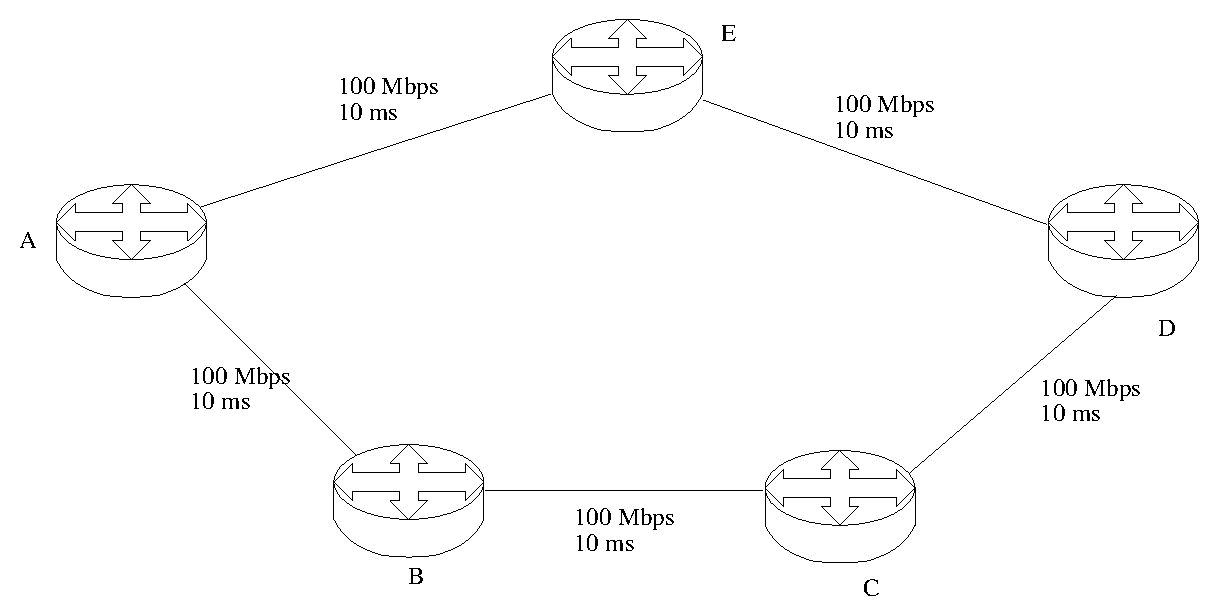
\includegraphics[width=\linewidth]{figures/traffic-engineering.eps}
\caption{Example scenario to explain traffic engineering.}
\label{fig:traffic-engineering}
\end{figure}

The best route between $A$ and $D$ is $A-E-D$.
It has the same bandwidth, less hops, and less total delay than the alternative path $A-B-C-D$.

A datagram-oriented network would choose the best route for all the packet.
Notice that this might not be the best of ideas.
If we direct a total of 100 Mbps (10 of VoIP + 90 of backup data) to 100 Mbps links, queues will build up, and delay, jitter and packet loss will be high.


